\documentclass[xetex,mathserif,serif]{beamer}
\usepackage{polyglossia}
\setdefaultlanguage[babelshorthands=true]{russian}
\usepackage{minted}
\usepackage{tabu}
\usepackage[11pt]{moresize}

\useoutertheme{infolines}

\usepackage{fontspec}
\setmainfont{FreeSans}
\newfontfamily{\russianfonttt}{FreeSans}

\usepackage{textpos}
\setlength{\TPHorizModule}{1cm}
\setlength{\TPVertModule}{1cm}

\definecolor{links}{HTML}{2A1B81}
\hypersetup{colorlinks,linkcolor=,urlcolor=links}

\tabulinesep=0.7mm

\title{Архитектурные аспекты сетевой безопасности}
\subtitle{Часть 1: Шифры и подписи}
\author[Юрий Литвинов]{Юрий Литвинов \newline \textcolor{gray}{\small\texttt{yurii.litvinov@gmail.com}}}

\newcommand{\attribution}[1] {
\vspace{-5mm}\begin{flushright}\begin{scriptsize}\textcolor{gray}{\textcopyright\, #1}\end{scriptsize}\end{flushright}
}

\date{20.05.2019г}

\begin{document}

	\frame{\titlepage}

	\section{Введение}

	\begin{frame}
		\frametitle{Сетевая безопасность}
		\begin{itemize}
			\item Почти все сервисы требуют авторизации и обеспечения безопасности
			\item Аутентификация --- установление личности (точнее, идентичности) участника взаимодействия
			\begin{itemize}
				\item Обычно взаимна
			\end{itemize}
			\item Авторизация --- установление прав на выполнение операции
			\item Шифрование --- обеспечение конфиденциальности передаваемой информации
			\item Также важны:
			\begin{itemize}
				\item Целостность --- злоумышлениик ничего не поменял
				\item Актуальность --- злоумышленник не проиграл старое сообщение
			\end{itemize} 
		\end{itemize}
	\end{frame}

	\begin{frame}
		\frametitle{Некоторые соображения}
		\begin{itemize}
			\item Основные уязвимости в современных системах не технические по характеру
			\item Большинство попыток взлома --- изнутри организации
			\item Сетевая безопасность --- игра против живого, умного и часто хорошо оснащённого противника
			\begin{itemize}
				\item Задача средств безопасности --- не сделать взлом невозможным, а сделать его нерентабельным
			\end{itemize}
			\item За протоколами безопасности стоит большая наука
			\begin{itemize}
				\item Придумать свой хитрый шифр или протокол аутентификации в общем случае очень плохая идея
			\end{itemize} 
			\item tradeoff между безопасностью и удобством использования
		\end{itemize}
	\end{frame}

	\section{Шифрование}

	\begin{frame}
		\frametitle{Шифрование}
		\begin{center}
			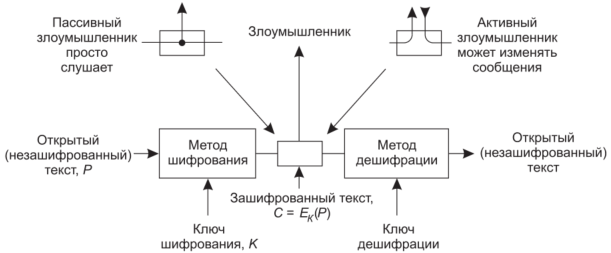
\includegraphics[width=0.6\textwidth]{cryptography.png}
			\attribution{Э. Таненбаум}
		\end{center}
		\begin{itemize}
			\item Алгоритм шифрования считается известным, секретен только ключ
			\item Усложнение алгоритма шифрования не всегда повышает криптостойкость
		\end{itemize}
		\begin{textblock}{2}(0,-6)
			
\includegraphics[width=\textwidth]{youAreBeingWatched.png}
		\end{textblock}
	\end{frame}

	\subsection{Шифрование с симметричным ключом}

	\begin{frame}
		\frametitle{Шифрование с симметричным ключом}
		\begin{itemize}
			\item Data Encryption Standard (DES, Triple DES)
			\item Advanced Encryption Standard (AES, он же Rijndael)
		\end{itemize}
		\begin{center}
			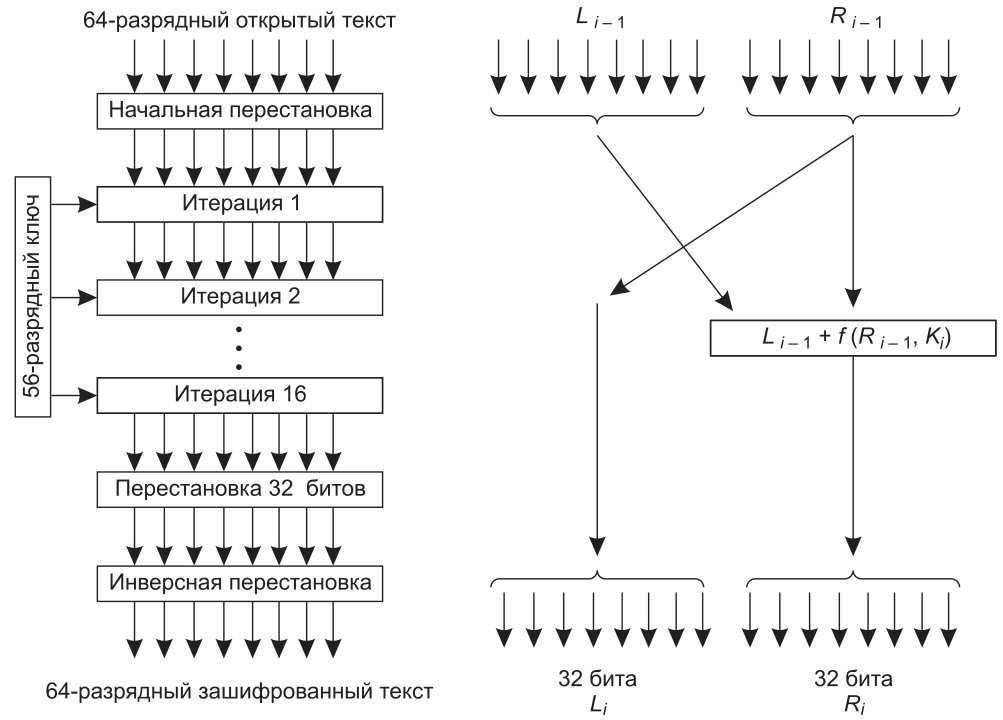
\includegraphics[width=0.6\textwidth]{des.png}
			\attribution{Э. Таненбаум}
		\end{center}
	\end{frame}

	\subsection{Режимы шифрования}

	\begin{frame}
		\frametitle{Режимы шифрования, ECB}
		\begin{itemize}
			\item Electronic Code Book --- один ключ применяется ко всем блокам
			\begin{itemize}
				\item Быстро, надёжно, но не криптостойко
			\end{itemize}
		\end{itemize}
		\begin{center}
			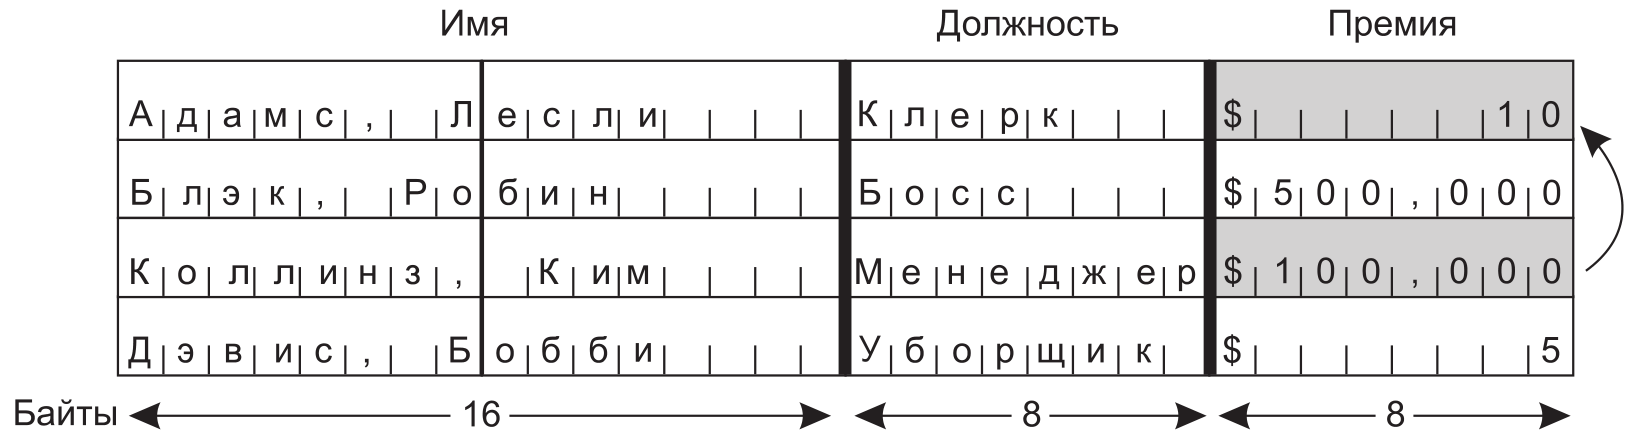
\includegraphics[width=0.85\textwidth]{ecbAttack.png}
			\attribution{Э. Таненбаум}
		\end{center}
	\end{frame}

	\begin{frame}
		\frametitle{Режимы шифрования, CBC}
		\begin{itemize}
			\item Cipher Block Chaining --- xor-им следующий блок с зашифрованным предыдущим перед шифровкой
			\begin{itemize}
				\item Более криптостоек, не устойчив к ошибкам передачи
				\item Initialization Vector (IV)
			\end{itemize}
		\end{itemize}
		\begin{center}
			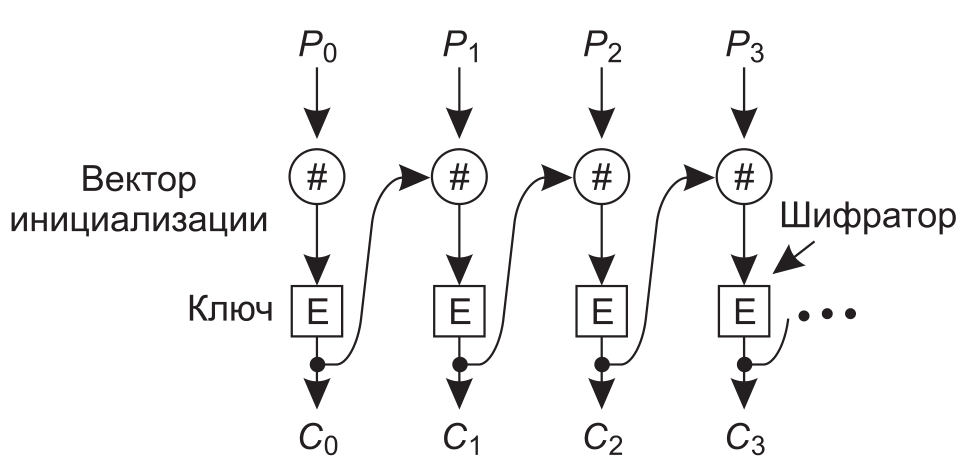
\includegraphics[width=0.6\textwidth]{cbc.png}
			\attribution{Э. Таненбаум}
		\end{center}
	\end{frame}

	\begin{frame}
		\frametitle{Режимы шифрования, SCM}
		\begin{itemize}
			\item Stream Cipher Mode --- шифруем IV ключом снова и снова, генерируя ключ бесконечной длины
			\begin{itemize}
				\item И xor-им его с шифруемым текстом
				\item Устойчив к ошибкам передачи, довольно быстр
				\item Уязвим к Keystream Reuse Attack ($(P_0 \oplus K_0) \oplus (Q_0 \oplus K_0)$)
			\end{itemize}
		\end{itemize}
		\begin{center}
			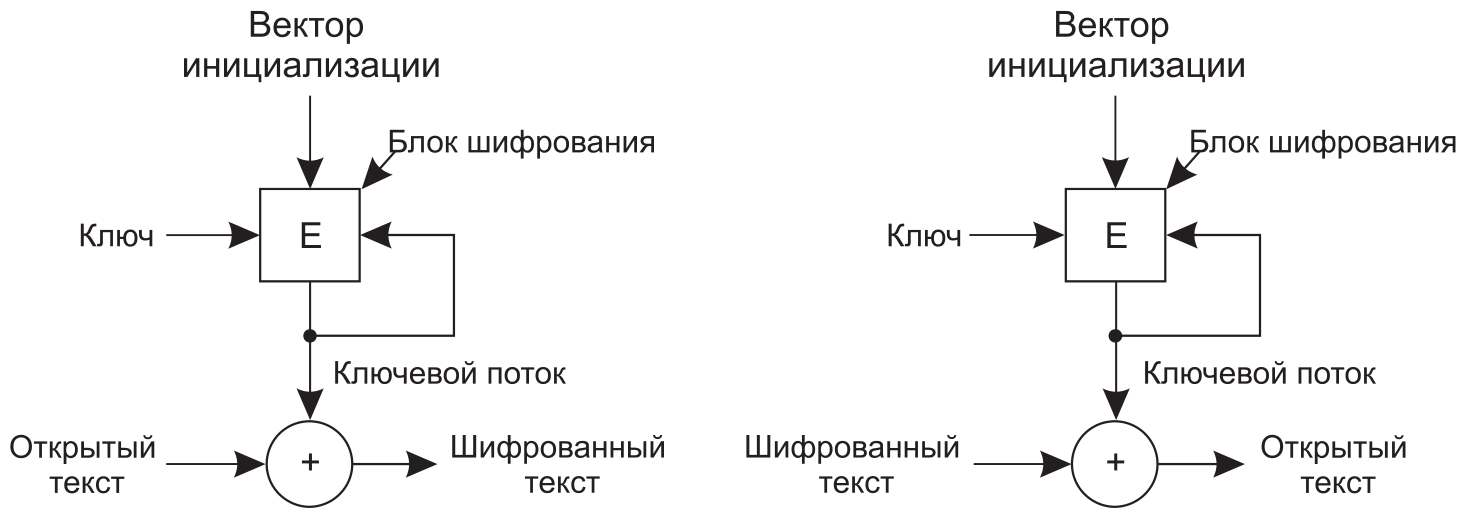
\includegraphics[width=0.85\textwidth]{scm.png}
			\attribution{Э. Таненбаум}
		\end{center}
	\end{frame}

	\begin{frame}
		\frametitle{Режимы шифрования, Counter Mode}
		\begin{itemize}
			\item Counter Mode --- шифруем $IV + i$ для каждого $i$-го блока
			\begin{itemize}
				\item И xor-им его с шифруемым текстом
				\item Для произвольного доступа к зашифрованным блокам
			\end{itemize}
		\end{itemize}
		\begin{center}
			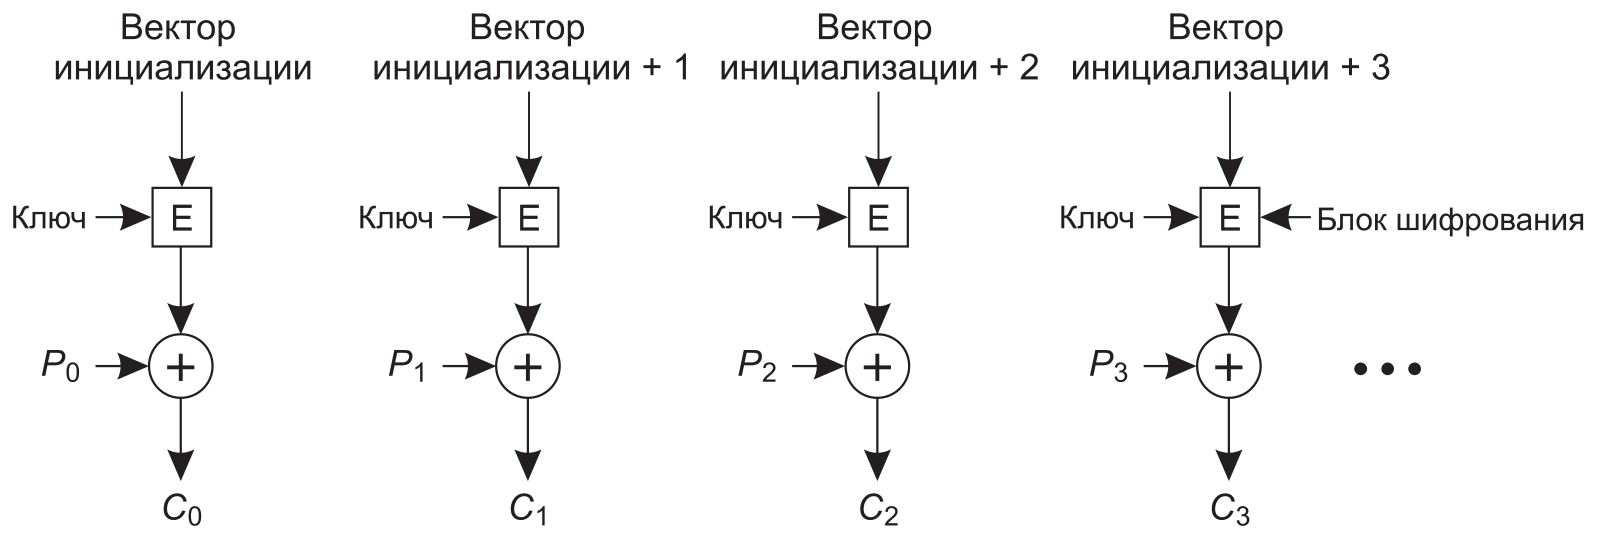
\includegraphics[width=0.85\textwidth]{cm.png}
			\attribution{Э. Таненбаум}
		\end{center}
	\end{frame}

	\subsection{Шифрование с открытым ключом}

	\begin{frame}
		\frametitle{Шифрование с открытым ключом}
		\framesubtitle{Или почему нельзя отдать ключи от Telegram}
		\begin{itemize}
			\item Алгоритм делится на две части, D и E, так, что D(E(P)) = P
			\item D очень сложно получить по E
			\begin{itemize}
				\item Например, найти простые сомножители огромного числа или дискретный логарифм по заданному модулю
			\end{itemize}
			\item E не ломается атакой ``произвольного открытого текста''
			\item D (ключ от D) держится в секрете, E выкладывается в открытый доступ
			\item Если Боб хочет послать Алисе сообщение, он берёт её открытый ключ $E_A$, шифрует им сообщение $P$ и отправляет Алисе
			\item Алиса дешифрует сообщение, вычисляя $D_A(E_A(P))$
			\item У каждого пользователя своя пара ключей
			\item Алгоритмы: RSA, ElGamal, эллиптические шифры
		\end{itemize}
	\end{frame}

	\begin{frame}
		\frametitle{Конкретно Telegram}
		\begin{itemize}
			\item Криптопротокол MTProto
			\begin{itemize}
				\item AES + Диффи-Хеллман
			\end{itemize}
			\item ``Секретные чаты'' отключены по умолчанию
			\begin{itemize}
				\item Для удобства --- позволяют только обмен ``устройство-устройство''
			\end{itemize}
			\item Без ``секретных чатов'' ничего секретного в Telegram нет
			\begin{itemize}
				\item Коммуникации с сервером шифруются, но если сервер взломают, то всё
			\end{itemize}
			\item ``Атака присутствия''
		\end{itemize}
	\end{frame}

	\section{Цифровые подписи}

	\begin{frame}
		\frametitle{Цифровые подписи, задачи}
		\begin{itemize}
			\item Получатель может установить личность отправителя
			\item Отправитель не может отрицать, что он подписал сообщение
			\item Получатель не может сам подделать сообщение и сделать вид, что его послал отправитель
		\end{itemize}
	\end{frame}

	\begin{frame}
		\frametitle{Цифровые подписи, реализация}
		\begin{center}
			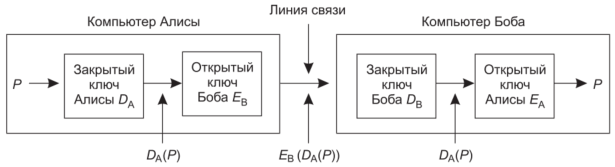
\includegraphics[width=0.7\textwidth]{signature.png}
			\attribution{Э. Таненбаум}
		\end{center}
		\begin{itemize}
			\item Надо, чтобы $D(E(P)) = P$ (это так для большинства криптосхем)
			\item Шифровать всё сообщение слишком медленно
			\item Message Digest-ы --- хорошие хеши сообщений
			\begin{itemize}
				\item MD5, SHA-1
			\end{itemize}
			\item Подписывается только хеш, это почти так же криптостойко, но в сотни раз быстрее
		\end{itemize}
	\end{frame}

	\begin{frame}
		\frametitle{SHA-1}
		\begin{itemize}
			\item Считается блоками по 512 бит, возвращает 160-битный дайджест
			\item Изменение в одном бите входа даёт совершенно другой выход
			\item Если известен $P$, очень сложно найти такой $P\ '$, что $MD(P\ ') = MD(P)$
		\end{itemize}
		\begin{center}
			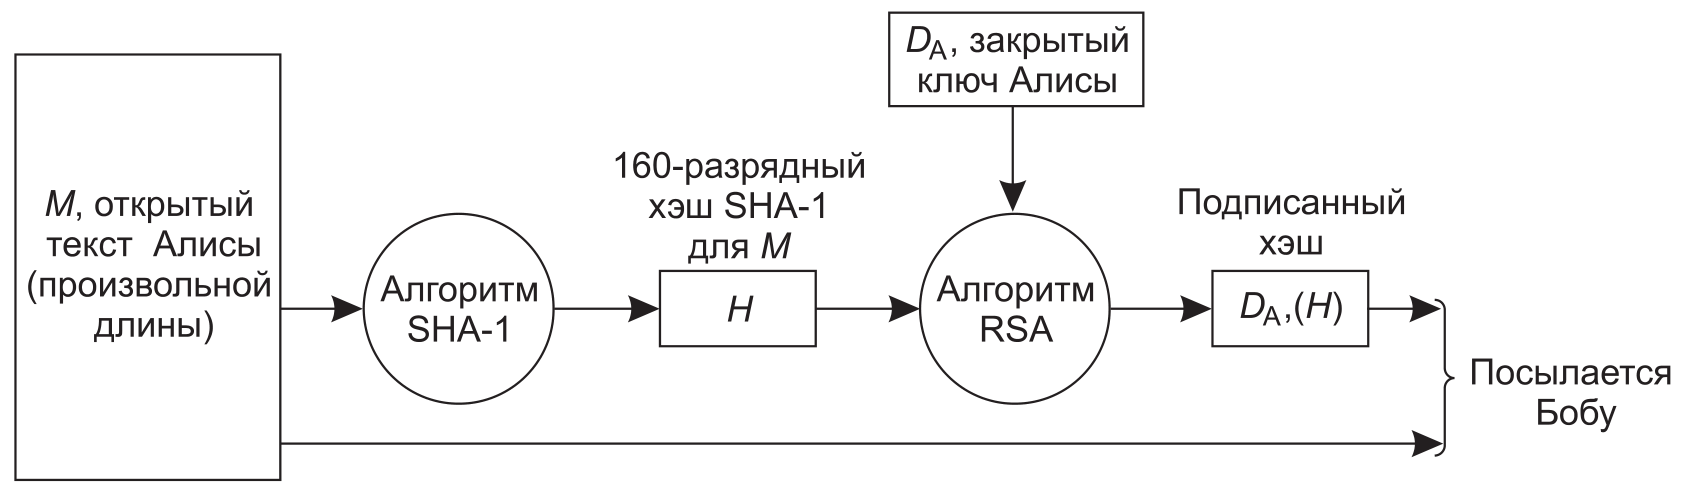
\includegraphics[width=0.85\textwidth]{sha1Signature.png}
			\attribution{Э. Таненбаум}
		\end{center}
	\end{frame}

	\begin{frame}
		\frametitle{Атака дней рождения}
		\begin{scriptsize}
Уважаемый господин декан,

\vspace{3mm}

Это [письмо | обращение] отражает мое [искреннее | откровенное] [мнение | суждение] о проф. Томе Уилсоне, являющемся [кандидатом | претендентом] на профессорскую должность в [настоящее время | этом году]. Я [знакома | работала] с проф. Уилсоном в течение [почти | около] шести лет. Он является [слабым | недостаточно талантливым] [исследователем | ученым], почти не известным в той области науки, которой он занимается. В его работах практически не заметно понимания [ключевых | главных] [проблем | вопросов] современности.

\vspace{3mm}

[Более | Кроме] того, он также не является сколько-нибудь [уважаемым | ценимым] [преподавателем | педагогом]. Его студенты дают его [занятиям | лекциям] [самые низкие | негативные] оценки. Он самый непопулярный [преподаватель | учитель] нашей кафедры, [славящийся | печально известный] своей [привычкой | склонностью] [высмеивать | ставить в неудобное положение] студентов, осмелившихся задавать вопросы на его [лекциях | занятиях].

\vspace{3mm}

% [Кроме | Помимо] того, [гранты | контракты] проф. Уилсона [почти | практически] не пополняют [фондов | финансовых запасов] нашей кафедры. Если не удастся быстро найти новый источник финансирования, [мы будем вынуждены | нам придется] [закрыть | прекратить] [много | ряд] [важных | специальных] программ, [таких как | среди которых] государственная программа 2000 года. К сожалению, при таких [условиях | обстоятельствах] я не могу [предлагать | рекомендовать] его вам на эту должность.
		\end{scriptsize}
	\end{frame}

\end{document}